\chapter{Approximate Bayesian Computation}

Lacey Knowles studied grasshoppers in the genus {\it Melanopus}. She
collected 1275bp of DNA sequence data from cytochrome oxidase I (COI)
from 124 individuals of {\it M. oregonensis\/} and two outgroup
speices. The specimens were collected from 15 ``sky-island'' sites in
the northern Rocky Mountains~(see Figure~\ref{fig:sky-islands};
\cite{Knowles-2001}). Two alternative hypotheses had been proposed to
describe the evolutionary relationships among these
grasshoppers~(refer to Figure~\ref{fig:divergence-hypotheses} for a
pictorial representation):\index{Melanopus@\textit{Melanopus}}

\begin{figure}
\begin{center}
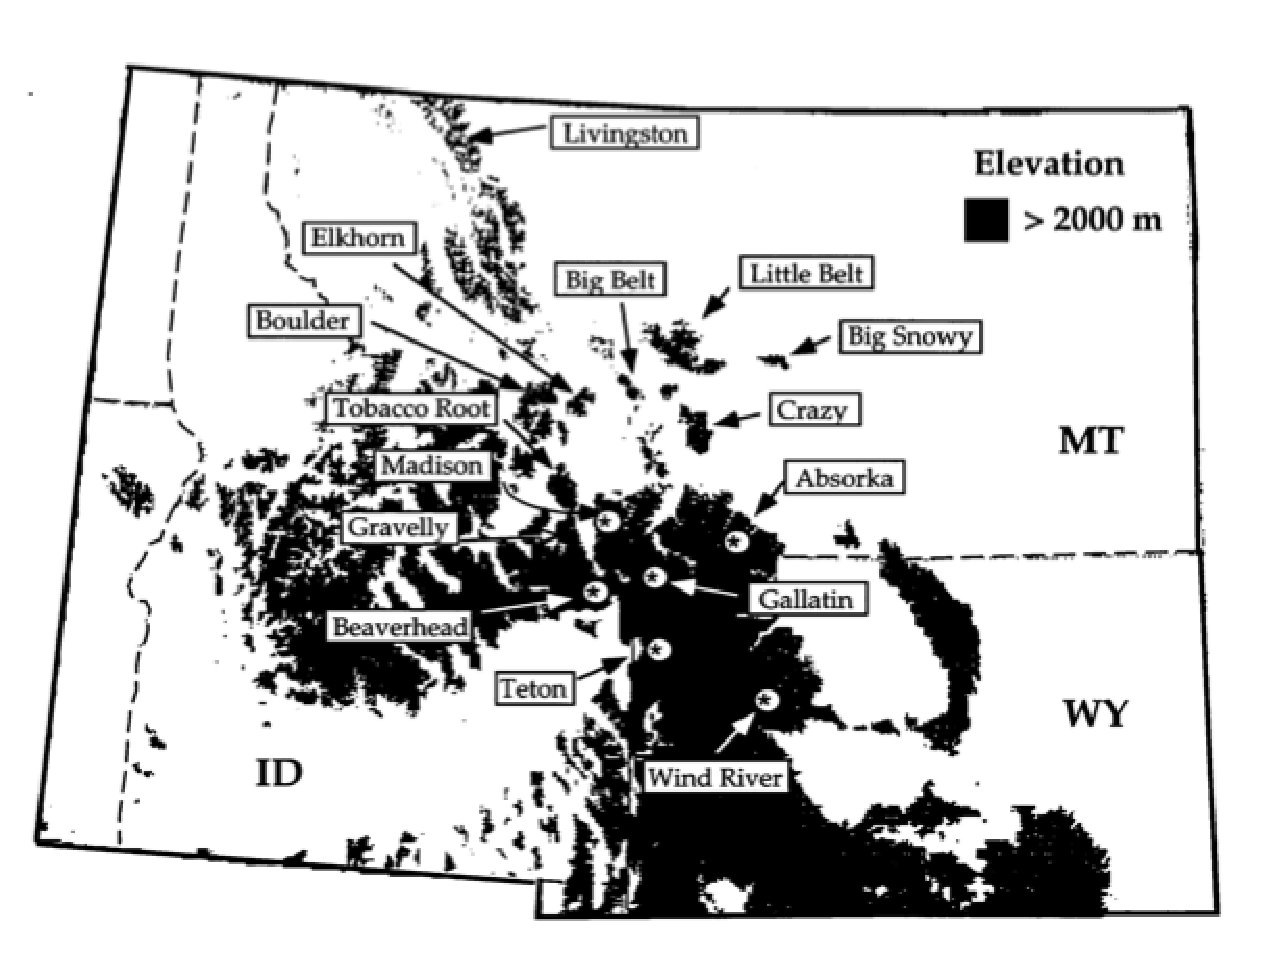
\includegraphics[height=6cm]{sky-islands.eps}
\end{center}
\caption{Collection sites for {\it Melanopus oregonensis\/} in the
  northern Rocky Mountains~(from~\cite{Knowles-2001}).}\label{fig:sky-islands}
\end{figure}

\begin{itemize}

\item {\bf Widespread ancestor}: The existing populations might represent
  independently derived remnants of a single, widespread
  population. In this case all of the populations would be equally
  related to one another.

\item {\bf Multiple glacial refugia}: Populations that shared the same
  refugium will be closely related while those that were in different
  refugia will be distantly related.

\end{itemize}

\begin{figure}
\begin{center}
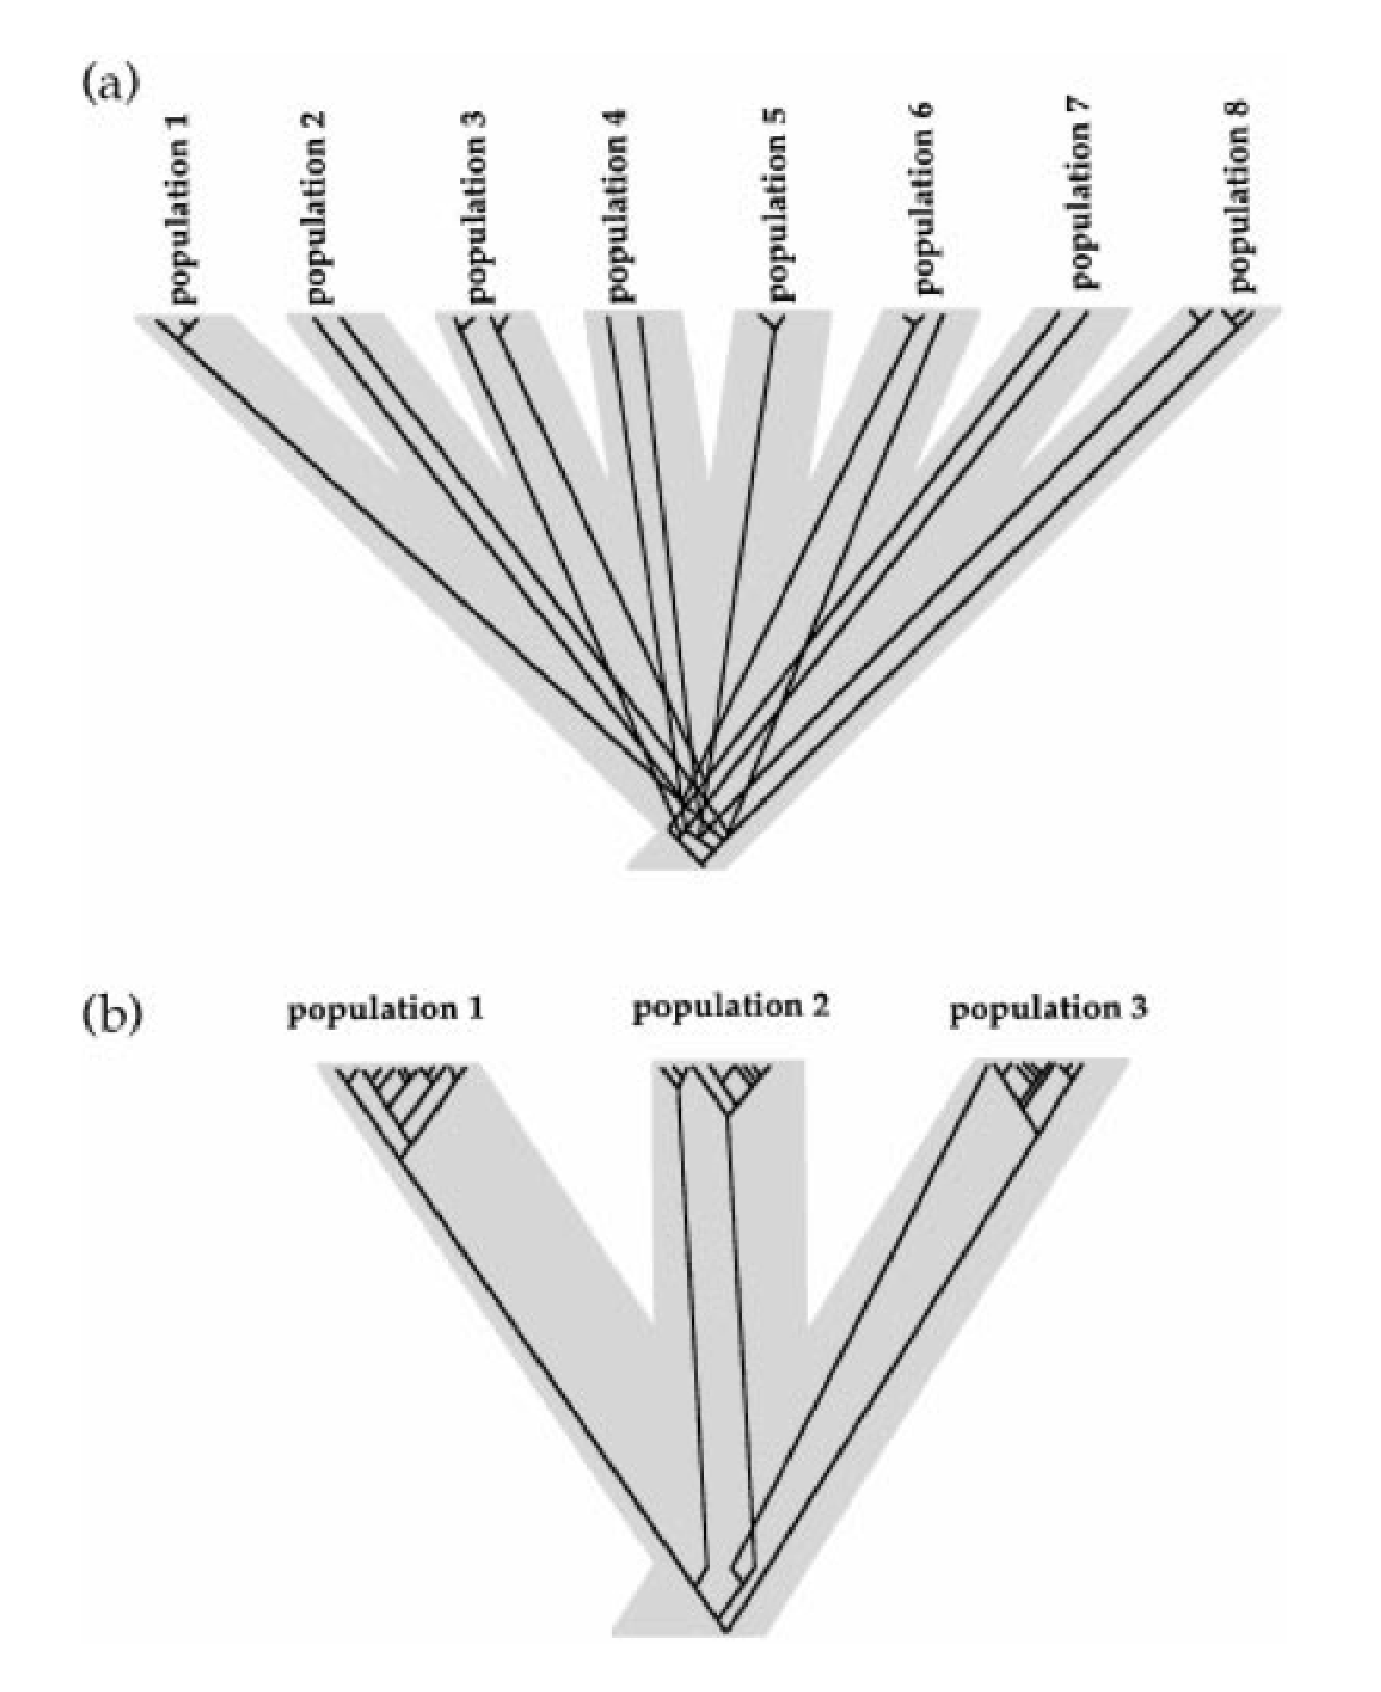
\includegraphics[height=6cm]{divergence-hypotheses.eps}
\end{center}
\caption{Pictorial representations of the ``widespread ancestor''
  (top) and ``glacial refugia'' (bottom)
  hypotheses~(from~\cite{Knowles-2001}).}\label{fig:divergence-hypotheses}
\end{figure}

As is evident from Figure~\ref{fig:divergence-hypotheses}, the two
hypotheses have very different consequences for the coalescent history
of alleles in the sample. Since the interrelationships between
divergence times and time to common ancestry differ so markedly
between the two scenarios, the pattern of sequence differences found
in relation to the geographic distribution will differ greatly between
the two scenarios. 

Using techniques described in Knowles and
Maddison~\cite{Knowles-Maddison-2002}, Knowles simulated gene trees
under the widespread ancestor hypothesis. She then placed them within
a population tree representing the multiple glacial refugia hypothesis
and calculated a statistic, $s$, that measures the discordance between
a gene tree and the population tree that contains it. This gave her a
distribution of $s$ under the widespread ancestor hypothesis. She
compared the $s$ estimated from her actual data with this distribution
and found that the observed value of $s$ was only 1/2 to 1/3 the size
of the value observed in her simulations.\footnote{The discrepancy was
  largest when divergence from the widespread ancestor was assumed to
  be very recent.} Let's unpack that a bit. 

\begin{itemize}

\item Knowles estimated the the phylogeny of the haplotypes in her
  sample. $s$ is the estimated minimum number of among-population
  migration events necessary to account for where haplotypes are
  currently found given the inferred
  phylogeny~\cite{Slatkin-Maddison-1989}. Let's call the $s$ estimated
  from the data $s_{obs}$.

\item Then she simulated a neutral coalescence process in which the
  populations were derived from a single, widespread ancestral
  population. For each simulation she rearranged the data so that
  populations were grouped into separate refugia and estimated $s_{sim}$
  from the rearranged data, and she repeated this 100 times for
  several different times since population splitting.

\end{itemize}

\noindent The results are shown in
Figure~\ref{fig:knowles-s-values}. As you can see, the observed $s$
value is much smaller than any of those obtained from the coalescent
simulations. That means that the observed data require far fewer
among-population migration events to account for the observed
geographic distribution of haplotypes than would be expected with
independent origin of the populations from a single, widespread
ancestor. In short, Knowles presented strong evidence that her data
are not consistent with the widespread ancestor
hypothesis.\index{statistical phylogeography!example}

\begin{figure}
\begin{center}
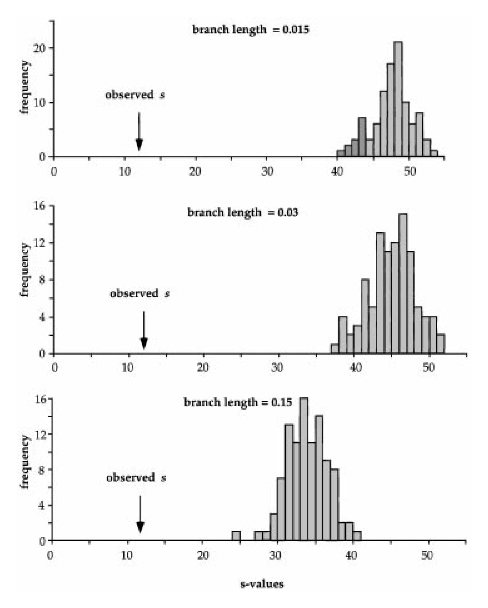
\includegraphics[height=10cm]{knowles-s-values.eps}
\end{center}
\caption{Distribution of the observed minimum number of
  among-population migration events, $s$, and the expected minimum
  number of migration events under the ``widespread ancestor''
  hypothesis.~(from~\cite{Knowles-2001}).}\label{fig:knowles-s-values}
\end{figure}

\section*{Approximate Bayesian computation: motivation}\index{ABC}\index{Approximate Bayesian Computation}

Approximate Bayesian Computation (ABC for short), extends the basic
idea we've just seen to consider more complicated scenarios. The {\tt
  IMa} approach developed by Nielsen, Wakely, and Hey is potentially
{\it very\/} flexible and {\it very\/}
powerful~\cite{Hey-Nielsen-2004,Hey-Nielsen-2007,Nielsen-Wakeley-2001}. It
allows for non-equilibrium scenarios in which the populations from
which we sampled diverged from one another at different times, but
suppose that we think our populations have dramatically increased in
size over time (as in humans) or dramatically changed their
distribution (as with an invasive species). Is there a way to use
genetic data to gain some insight into those processes? Would I be
asking that question if the answer were ``No''?

\section*{An example}

Let's change things up a bit this time and start with an example of a
problem we'd like to solve first. Once you see what the problem is,
then we can talk about how we might go about solving it. The case
we'll discuss is the case of the cane toad, {\it Bufo marinus}, in
Australia.\index{Bufo@\textit{Bufo}!\textit{marinus}}

You may know that the cane toad is native to the American tropics. It
was purposely introduced into Australia in 1935 as a biocontrol agent,
where it has spread across an area of more than 1 million km$^2$. Its
range is still expanding in northern Australia and to a lesser extent
in eastern
Australia~(Figure~\ref{fig:cane-toad-expansion}).\footnote{All of this
  information is from the introduction to~\cite{Estoup-etal-2004}.}
Estoup et al.~\cite{Estoup-etal-2004} collected microsatellite data
from 30 individuals in each of 19 populations along roughly linear
transects in the northern and eastern expansion areas.

\begin{figure}
\begin{center}
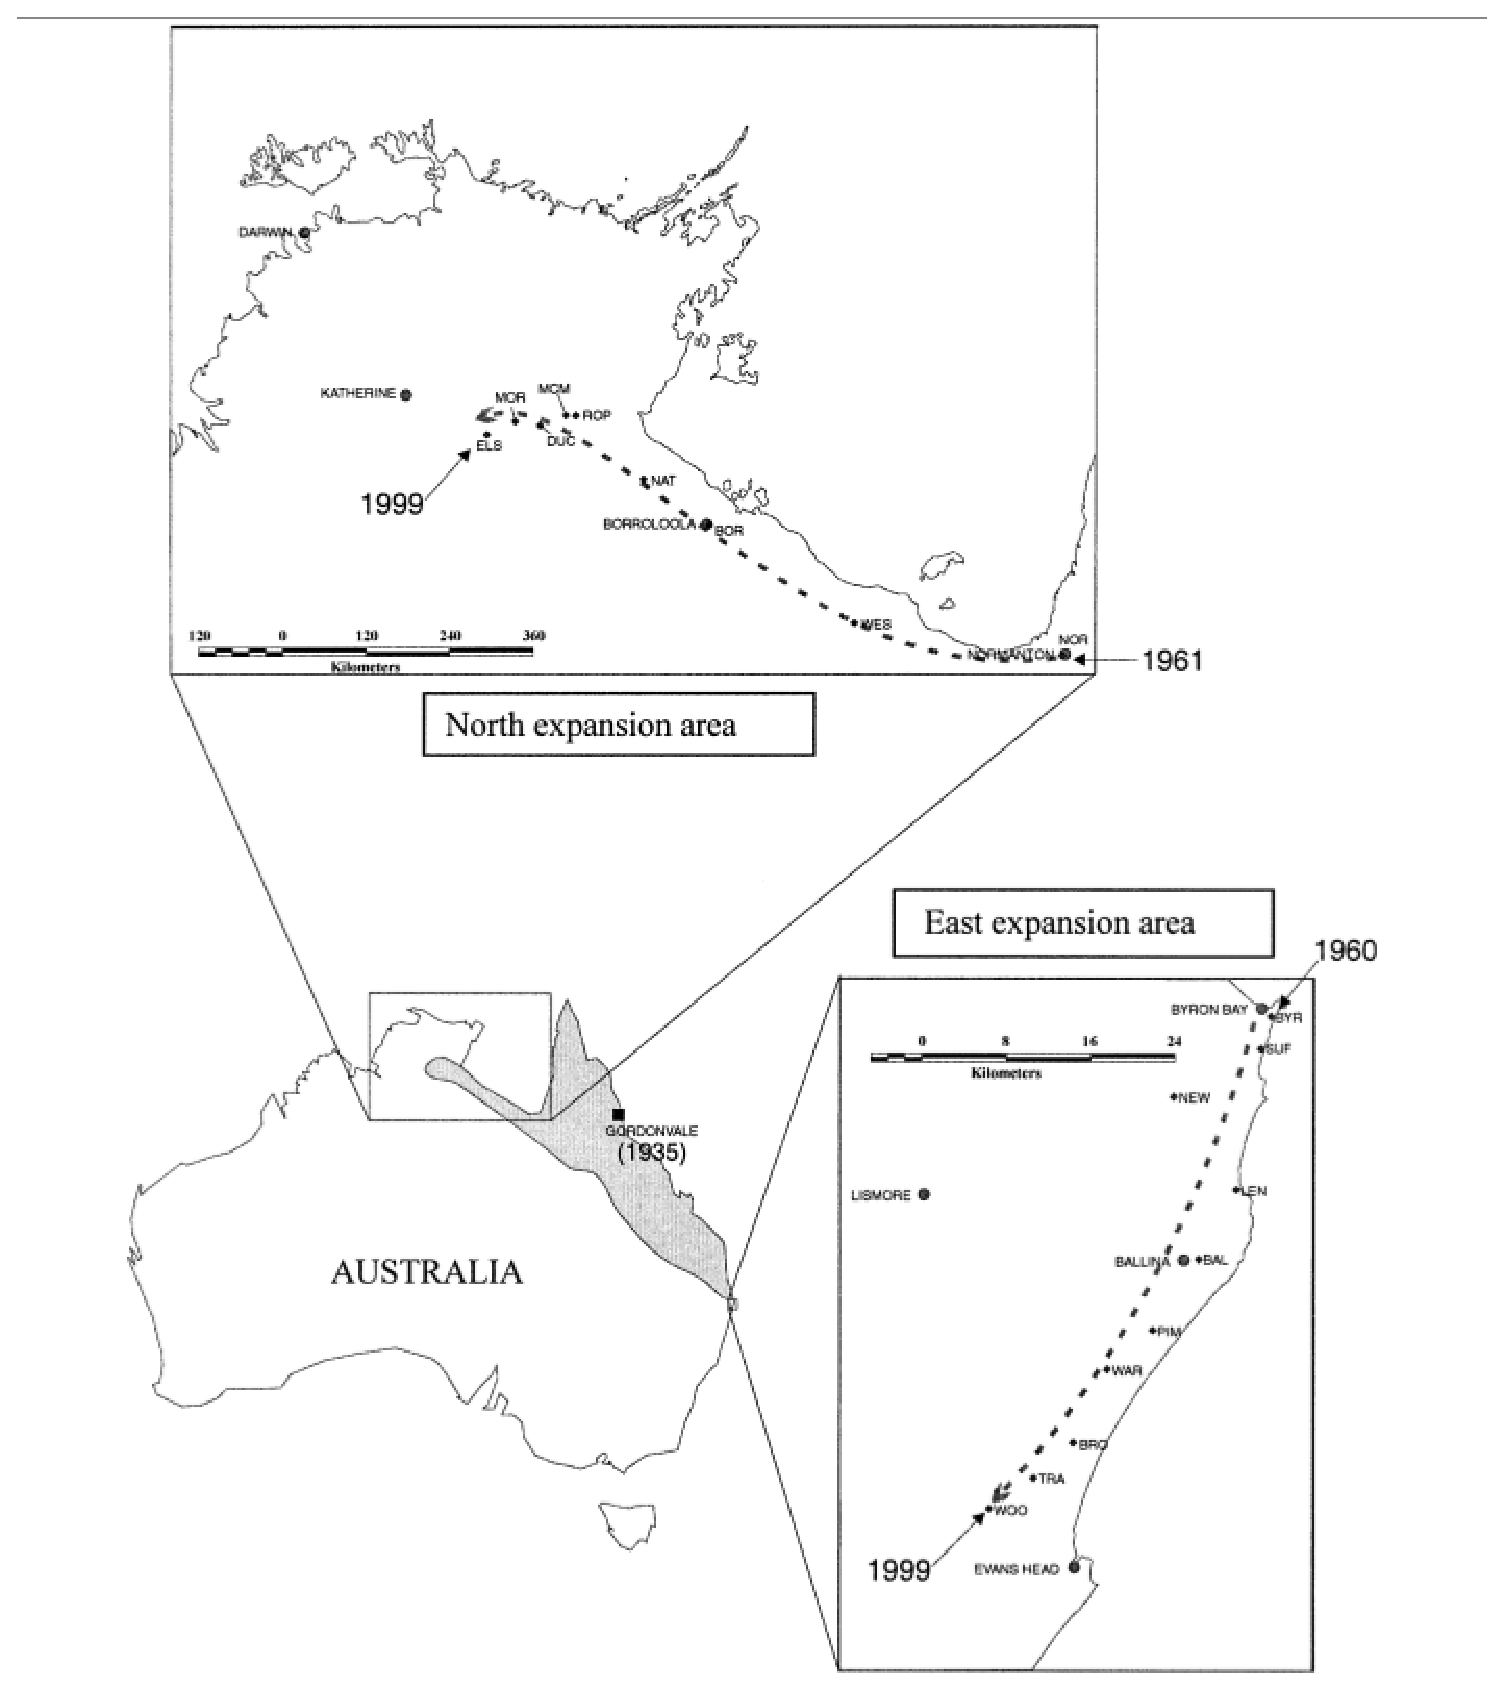
\includegraphics[width=6.0in]{cane-toad-expansion.eps}
\end{center}
\caption{Maps showing the expansion of the cane toad population in
  Australia since its introduction in 1935~(from~\cite{Estoup-etal-2004}).}\label{fig:cane-toad-expansion}
\end{figure}

With these data they wanted to distinguish among five possible
scenarios describing the geographic spread:

\begin{itemize}

\item {\bf Isolation by distance}: As the expansion proceeds, each new
  population is founded by or immigrated into by individuals with a
  probability proportional to the distance from existing populations.

\item {\bf Differential migration and founding}: Identical to the
  preceding model except that the probability of founding a population
  may be different from the probability of immigration into an
  existing population.

\item {\bf ``Island'' migration and founding}: New populations are
  established from existing populations without respect to the
  geographic distances involved, and migration occurs among
  populations without respect to the distances involved.

\item {\bf Stepwise migration and founding with founder events}: Both
  migration and founding of populations occurs only among immediately
  adjacent populations. Moreover, when a new population is
  established, the number of individuals involved may be very small.

\item {\bf Stepwise migration and founding without founder events}:
  Identical to the preceding model except that when a population is
  founded its size is assumed to be equal to the effective population
  size. 

\end{itemize}

That's a pretty complex set of scenarios. Clearly, you could use {\tt
  Migrate} or {\tt IMa2} to estimate parameters from the data Estoup
et al.~\cite{Estoup-etal-2004} report, but would those parameters
allow you to distinguish those scenarios? Not in any straightforward
way that I can see. Neither {\tt Migrate} nor {\tt IMa2} distinguishes
between founding and migration events for example. And with {\tt IMa2}
we'd have to specify the relationships among our sampled populations
before we could make any of the calculations. In this case we want to
test alternative hypotheses of population relationship. So what do we
do?

\section*{Approximate Bayesian Computation}\index{Approximate Bayesian Computation}

Well, in principle we could take an approach similar to what {\tt
  Migrate} and {\tt IMa2} use. Let's start by reviewing what we did
last time\footnote{More accurately, what Peter Beerli, Joe
  Felsenstein, Rasmus Nielsen, John Wakeley, and Jody Hey did.} with
{\tt Migrate} and {\tt IMa2}. In both cases, we knew how to simulate
data given a set of mutation rates, migration rates, local effective
population sizes, and times since divergence. Let's call that whole,
long string of parameters $\xi$ and our big, complicated data set
$X$. If we run enough simulations, we can keep track of how many of
those simulations produce data identical to the data we
collected. With those results in hand, we can estimate $P(X|\xi)$,
the likelihood of the data, as the fraction of simulations that
produce data identical to the data we collected.\footnote{The actual
  implementation is a bit more involved than this, but that's the
  basic idea.} In principle, we could take the same approach in this,
much more complicated, situation. But the problem is that there are an
astronomically large number of different possible coalescent histories
and different allelic configurations possible with any one population
history both because the population histories being considered are
pretty complicated and because the coalescent history of every locus
will be somewhat different from the coalescent history at other
loci. As a result, the chances of getting {\it any\/} simulated
samples that match our actual samples is virtually nil, and we can't
estimate $P(X|\xi)$ in the way we have so far.

Approximate Bayesian computation is an approach that allows us to get
around this problem. It was introduced by Beaumont et
al.~\cite{Beaumont-etal-2002} precisely to allow investigators to get
approximate estimates of parameters and data likelihoods in a Bayesian
framework. Again, the details of the implementation get pretty
hairy,\footnote{You're welcome to read the Methods
  in~\cite{Beaumont-etal-2002}, and feel free to ask questions if
  you're interested. I have to confess that there's a decent chance I
  won't be able to answer your question until I've done some further
  studying. I've only used ABC a little, and I haven't used it for
  anything that I've published{\dash}yet.} but the basic idea is relatively
straightforward.\footnote{OK. This maybe calling it ``relatively
  straightforward'' is misleading. Even this simplified outline is
  fairly complicated, but compared to some of what you've already
  survived in this course, it may not look too awful.}

\begin{enumerate}

\item Calculate ``appropriate'' summary statistics for your data set,
  e.g., pairwise estimates of $\phi_{ST}$ (possibly one for every
  locus if you're using microsatellite or SNP data), estimates of
  within population diversity, counts of the number of segregating
  sites~(for nucleotide sequence data, both within each population and
  across the entire sample) or counts of the number of segregating
  alleles~(for microsatellite data). Call that set of summary
  statistics $S$.

\item Specify a prior distribution for the unknown parameters, $\xi$.

\item Pick a random set of parameter values, $\xi'$ from the prior
  distribution and simulate a data set for that set of parameter
  values.

\item Calculate the same summary statistics for the simulated
  data set as you calculated for your actual data. Call that set of
  statistics $S'$. 

\item Calculate the distance between $S$ and $S'$.\footnote{You could
    use any one of a variety of different distance measures. A simple
    Euclidean distance might be useful, but you could also try
    something more complicated, like a Mahalanobis distance.} Call it
  $\delta$. If it's less than some value you've decided on,
  $\delta^*$, keep track of $S'$ and the associated $\xi'$ and
  $\delta$. Otherwise, throw all of them away and forget you ever saw
  them.

\item Return to step 2 and repeat until you you have accepted a large
  number of pairs of $S'$ and $\xi'$.

\end{enumerate}

Now you have a bunch of $S'$s and a bunch of $\xi'$s that produced
them. Let's label them $S_i$ and $\xi_i$, and let's remember what
we're trying to do. We're trying to estimate $\xi$ for our real
data. What we have from our real data is $S$. So far it seems as if
we've worked our computer pretty hard, but we haven't made any
progress. 

Here's where the trick comes in. Suppose we fit a regression to the
data we've simulated
\[
\xi_i = \alpha + S_i\beta + \epsilon \quad ,
\]
where $\alpha$ is an intercept, $\beta$ is a vector of regression
coefficients relating each of the summary statistics to $\xi$, and
$\epsilon$ is an error vector.\footnote{I know what you're thinking to
  yourself now. This doesn't sound very simple. Trust me. It is as
  simple as I can make it. The actual procedure involves local linear
  regression. I'm also not telling you how to go about picking
  $\delta$ or how to pick ``appropriate'' summary statistics. There's
  a fair amount of ``art'' involved in that.} Once we've fit this
regression, we can use it to predict what $\xi$ should be in our real
data, namely
\[
\xi = \alpha + S\beta \quad ,
\]
where the $S$ here corresponds to our observed set of summary
statistics. If we throw in some additional bells and whistles, we can
approximate the posterior distribution of our parameters. With that we
can get not only a point estimate for $\xi$, but also credible
intervals for all of its components.\index{Approximate Bayesian Computation!regression}

\section*{Back to the real world\footnote{Or at least something
    resembling the real world}}

OK. So now we know how to do ABC, how do we apply it to the cane toad
data. Well, using the additional bells and whistles I mentioned, we
end up with a whole distribution of $\delta$ for each of the scenarios
we try. The scenario with the smallest $\delta$ provides the best fit
of the model to the data. In this case, that corresponds to model 4,
the stepwise migration with founder model, although it is only
marginally better than model 1 (isolation by distance) and model 2
(isolation by distance with differential migration and founding) in
the northern expansion area~(Figure~\ref{fig:cane-toad-models}).\index{Bufo@\textit{Bufo}!\textit{marinus}}

\begin{figure}
\begin{center}
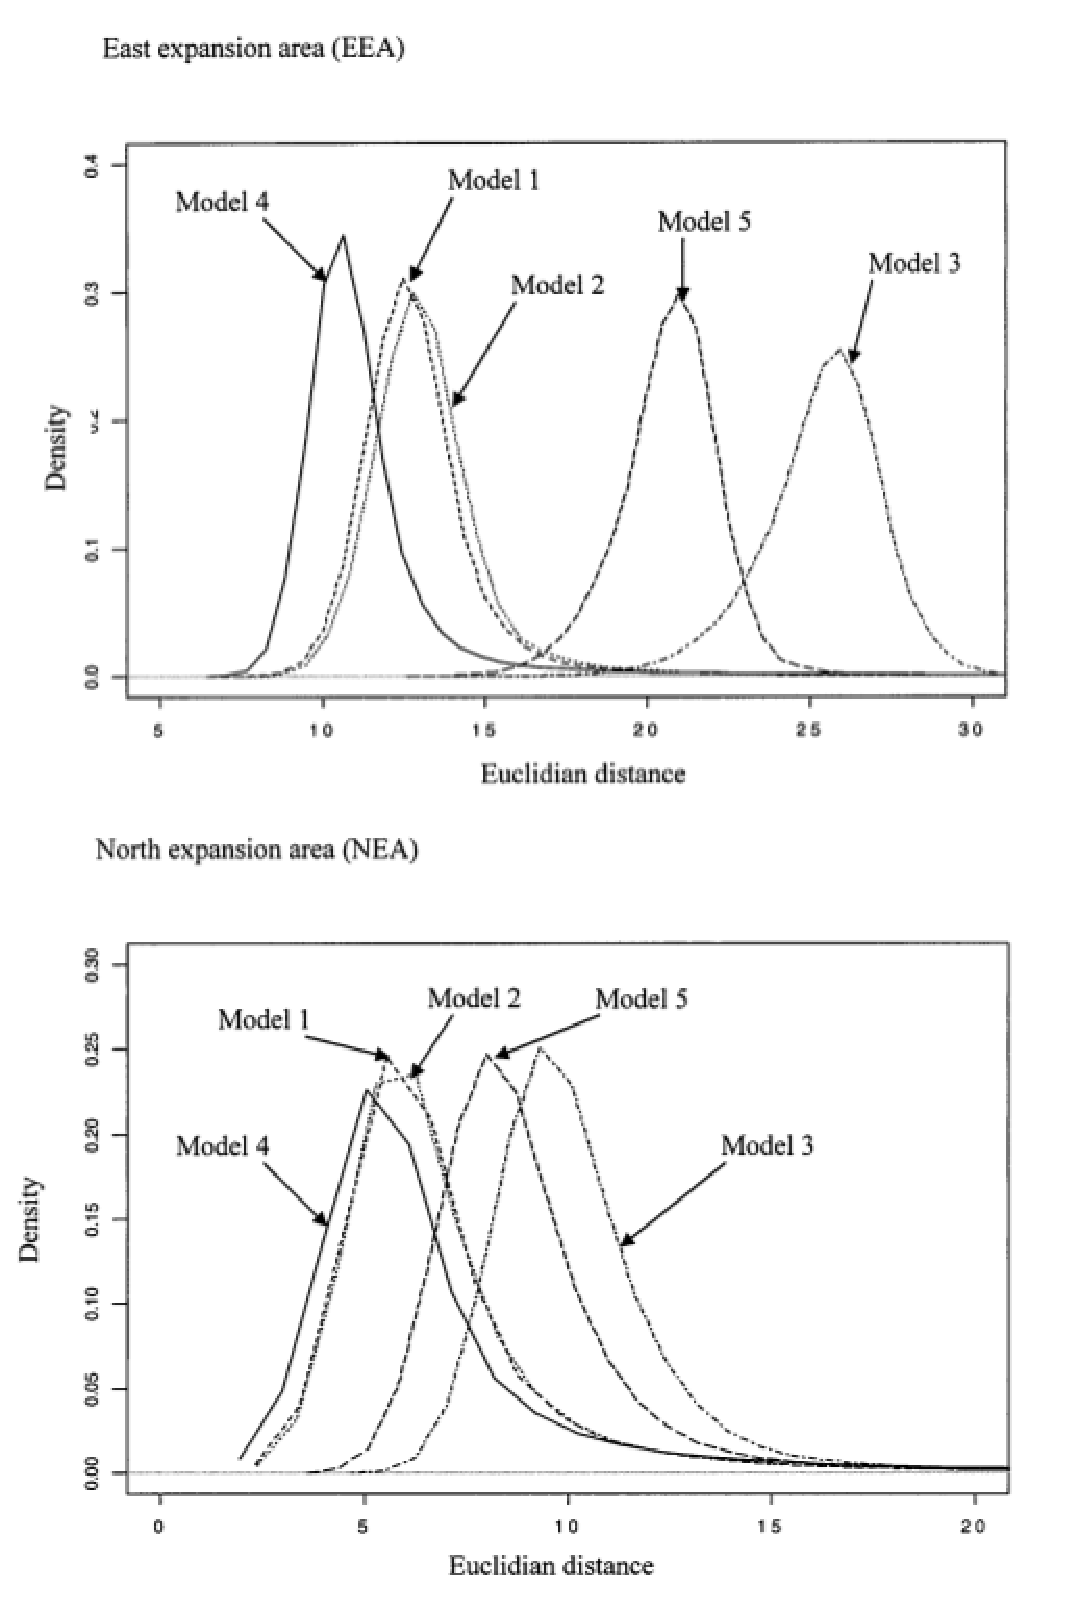
\includegraphics[width=4.5in]{cane-toad-models.eps}
\end{center}
\caption{Posterior distribution of $\delta$ for the five models
  considered in Estoup et al.~\cite{Estoup-etal-2004}.}\label{fig:cane-toad-models}
\end{figure}

Of course, we also have estimates for various parameters associated
with this model: 

\begin{itemize}

\item $N_{e_s}$: the effective population size when the population is
  stable.

\item $N_{e_f}$: the effective population size when a new population
  is founded.

\item $F_R$: the founding ratio, $N_{e_s}/N_{e_f}$.

\item $m$: the migration rate.

\item $N_{e_s}m$: the effective number of migrants per generation.

\end{itemize}

The estimates are summarized in Table~\ref{table:cane-toad}. Although
the credible intervals are fairly broad,\footnote{And notice that
  these are 90\% credible intervals, rather than the conventional 95\%
  credible intervals, which would be even broader.} there are a few
striking features that emerge from this analysis.

\begin{itemize}

\item Populations in the northern expansion area are larger, than
  those in the eastern expansion region. Estoup et
  al.~\cite{Estoup-etal-2004} suggest that this is consistent with
  other evidence suggesting that ecological conditions are more
  homogeneous in space and more favorable to cane toads in the north
  than in the east.

\item A smaller number of individuals is responsible for founding new
  populations in the east than in the north, and the ratio of
  ``equilibrium'' effective size to the size of the founding
  population is bigger in the east than in the north. (The second
  assertion is only weakly supported by the results.)

\item Migration among populations is more limited in the east than in
  the north. 

\end{itemize}

As Estoup et al.~\cite{Estoup-etal-2004} suggest, results like these
could be used to motivate and calibrate models designed to predict the
future course of the invasion, incorporating a balance between gene
flow (which can reduce local adaptation), natural selection, drift,
and colonization of new areas.

\begin{table}
\begin{center}
\begin{tabular}{ccr}
\hline\hline
Parameter & area & mean (5\%, 90\%) \\
\hline
$N_{e_s}$ & east & 744 (205, 1442) \\
         & north & 1685 (526, 2838) \\
$N_{e_f}$ & east & 78 (48, 118) \\
         & north & 311 (182, 448) \\
$F_R$    & east & 10.7 (2.4, 23.8) \\
         & north & 5.9 (1.6, 11.8) \\
$m$      & east & 0.014 ($6.0 \times 10^{-6}$, 0.064) \\
         & north & 0.117 ($1.4 \times 10^{-4}$, 0.664) \\
$N_{e_s}m$ & east & 4.7 (0.005, 19.9) \\
          & north & 188 (0.023, 883) \\
\hline
\end{tabular}
\end{center}
\caption{Posterior means and 90\% credible intervals for parameters of
  model 4 in the eastern and northern expansion areas of {\it Bufo
    marinus}.}\label{table:cane-toad}
\end{table}

\section*{Limitations of ABC}\index{Approximate Bayesian Computation!limitations}

If you've learned anything by now, you should have learned that there
is no perfect method. An obvious disadvantage of ABC relative to
either {\tt Migrate} or {\tt IMa2} is that it is much more
computationally intensive. 

\begin{itemize}

\item Because the scenarios that can be considered are much more
  complex, it simply takes a long time to simulate all of the data. 

\item In the last few years, one of the other disadvantages{\dash}that
  you had to know how to do some moderately complicated scripting to
  piece together several different packages in order to run
  analysis{\dash}has become less of a problem. {\tt popABC}
  (\url{http://code.google.com/p/popabc/} and {\tt DIYABC}
  (\url{http://www1.montpellier.inra.fr/CBGP/diyabc/}) make it {\it
    relatively\/} easy\footnote{Emphasis on ``relatively''.} to
  perform the simulations.

\item Selecting an appropriate set of summary statistics isn't easy,
  and it turns out that which set is most appropriate may depend on
  the value of the parameters that you're trying to estimate and the
  which of the scenarios that you're trying to compare is closest to
  the actual scenario applying to the populations from which you
  collected the data. Of course, if you knew what the parameter values
  were and which scenario was closest to the actual scenario, you
  wouldn't need to do ABC in the first place.

\item In the end, ABC allows you to compare a small number of
  evolutionary scenarios. It can tell you which of the scenarios
  you've imagined provides the best combination of fit to the data and
  parsimonious use of parameters (if you choose model comparison
  statistics that include both components), but it takes additional
  work to determine whether the model is adequate, in the sense that
  it does a good job of explaining the data. Moreover, even if you
  determine that the model is adequate, you can't exclude the
  possibility that there are other scenarios that might be equally
  adequate{\dash}or even better.

\end{itemize}

